\begin{frame}{The Convergence Challenge in MCMC}
	\begin{itemize}
		\item \textbf{Ideal goal}: Assess whether MCMC chains have converged
		\item \textbf{Fundamental problem}:
		      \begin{itemize}
			      \item In general, impossible to know for sure that there is no problem
			      \item But we can sometimes know for sure that there \textit{is} a problem
		      \end{itemize}
		\item \textbf{Two phases of MCMC}:
		      \begin{itemize}
			      \item Transient phase (burn-in): mixing time
			      \item Stationary phase: Monte Carlo estimation
		      \end{itemize}
	\end{itemize}

	\vspace{0.5cm}
	\begin{center}
		\tikz{
			\draw[thick, ->] (0,0) -- (8,0) node[right] {Iterations};
			\draw[thick] (0,-0.1) -- (0,0.1);
			\draw[thick] (3,-0.1) -- (3,0.1);
			\draw[copenhagenred, ultra thick] (0,0.5) -- (3,0.5);
			\draw[blue, ultra thick] (3,0.5) -- (8,0.5);
			\node at (1.5, 1) {\color{copenhagenred} Burn-in};
			\node at (5.5, 1) {\color{blue} Sampling};
		}
	\end{center}
\end{frame}

\begin{frame}{Why Convergence Matters}
	\textbf{Non-converged chains:}
	\begin{itemize}
		\item Biased estimates
		\item Incorrect uncertainty quantification
		\item Missing important modes
		\item Unreliable inference
	\end{itemize}

	\vspace{0.5cm}
	\begin{block}{Key Question}
		How can we diagnose whether our MCMC chains have converged to the target distribution?
	\end{block}
\end{frame}


\begin{frame}{Motivating example}
\begin{figure}
	\centering
	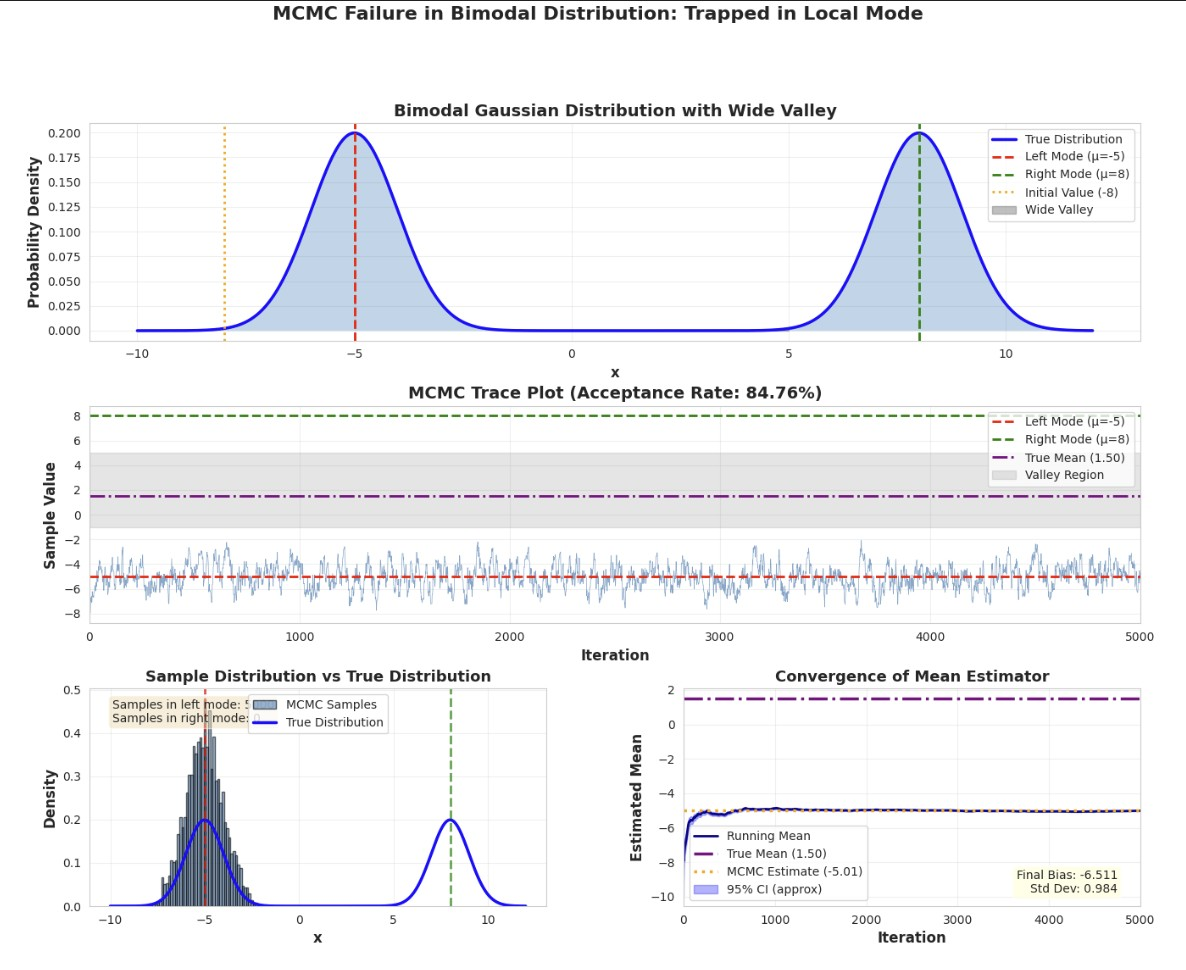
\includegraphics[width=0.6\textwidth]{bimodal.jpg}
	\caption{Trace plots of two MCMC chains that have not converged, illustrating the challenge of diagnosing convergence. Both chains appear stable but are sampling different regions of the parameter space.}
\end{figure}
\end{frame}

\begin{frame}{The Intuition Behind Gelman-Rubin}
	\begin{block}{Core Idea}
		If MCMC chains have converged to the target distribution, then:
		\begin{itemize}
			\item Multiple chains started from different points should look similar
			\item Between-chain variance $\approx$ Within-chain variance
		\end{itemize}
	\end{block}

		\textbf{Compare two sources of variance:}
		\begin{enumerate}
			\item \textcolor{blue}{Within-chain variance (W)}\\
					How much each chain varies
			\item \textcolor{red}{Between-chain variance (B)}\\
					How different chains are from each other
		\end{enumerate}
\end{frame}

\begin{frame}{Mathematical Foundation}
	Consider $M$ chains, each of length $T$:

	\begin{block}{Variance Decomposition}
		Total sum of squares = Inter-group + Intra-group
		$$\sum_{m=1}^M \sum_{t=1}^T (X_{m,t} - \bar{X}_{..})^2 =
			\textcolor{red}{\sum_{m=1}^M \sum_{t=1}^T (\bar{X}_m - \bar{X}_{..})^2} +
			\textcolor{blue}{\sum_{m=1}^M \sum_{t=1}^T (X_{m,t} - \bar{X}_m)^2}$$
	\end{block}

	\vspace{0.3cm}
	\begin{itemize}
		\item \textcolor{blue}{Intra-group} = Within-chain variance (W)
		\item \textcolor{red}{Inter-group} = Between-chain variance (B)
	\end{itemize}

	\vspace{0.3cm}
	Key insight: After convergence, both estimate the same target variance!
\end{frame}

\begin{frame}{The Gelman-Rubin Statistic}
	\begin{block}{Definition}
		$$\hat{R} = \sqrt{\frac{\hat{V}}{W}}$$
	\end{block}

	Where:
	\begin{align*}
		W       & = \frac{1}{M} \sum_{m=1}^M s_m^2 \quad \text{(average within-chain variance)}                   \\
		B       & = \frac{T}{M-1} \sum_{m=1}^M (\bar{X}_m - \bar{X}_{..})^2 \quad \text{(between-chain variance)} \\
		\hat{V} & = \frac{T-1}{T}W + \frac{1}{T}B \quad \text{(pooled variance estimate)}
	\end{align*}

	\vspace{0.3cm}
	\textbf{Interpretation:}
	\begin{itemize}
		\item $\hat{R} \approx 1$: Good convergence
		\item $\hat{R} > 1$: Chains haven't converged
		\item $\hat{R} \gg 1$: Serious convergence problems
	\end{itemize}
\end{frame}

\begin{frame}{Why It Works: The Variance Sandwich}
	\begin{center}
		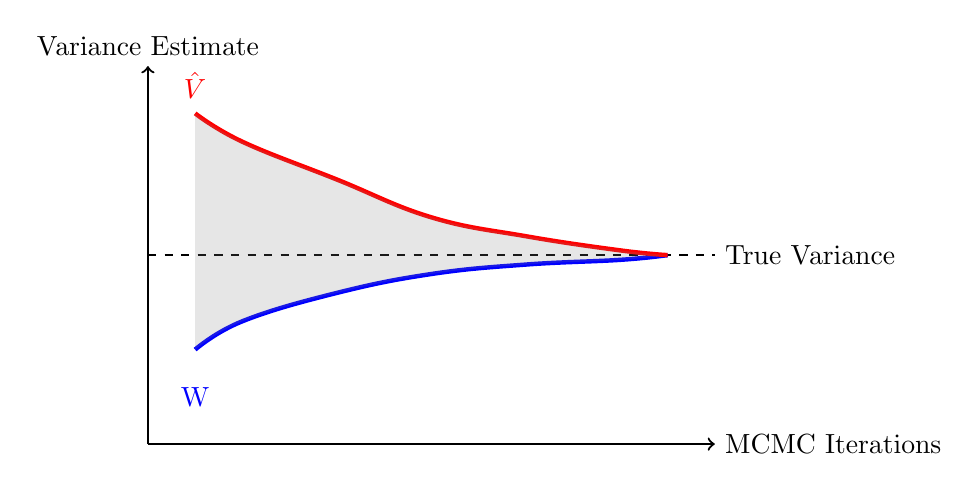
\begin{tikzpicture}[scale=1.2]
			% Draw variance evolution
			\draw[thick, ->] (0,0) -- (6,0) node[right] {MCMC Iterations};
			\draw[thick, ->] (0,0) -- (0,4) node[above] {Variance Estimate};

			% True variance line
			\draw[black, dashed, thick] (0,2) -- (6,2) node[right] {True Variance};

			% W line (underestimates initially)
			\draw[blue, ultra thick] plot[smooth, tension=0.7] coordinates
				{(0.5,1) (1,1.3) (2,1.6) (3,1.8) (4,1.9) (5,1.95) (5.5,2)};
			\node[blue] at (0.5,0.5) {W};

			% V line (overestimates initially)
			\draw[red, ultra thick] plot[smooth, tension=0.7] coordinates
				{(0.5,3.5) (1,3.2) (2,2.8) (3,2.4) (4,2.2) (5,2.05) (5.5,2)};
			\node[red] at (0.5,3.8) {$\hat{V}$};

			% Shaded area
			\fill[gray, opacity=0.2] (0.5,1) -- plot[smooth, tension=0.7] coordinates
				{(0.5,1) (1,1.3) (2,1.6) (3,1.8) (4,1.9) (5,1.95) (5.5,2)}
			-- (5.5,2) -- plot[smooth, tension=0.7] coordinates
				{(5.5,2) (5,2.05) (4,2.2) (3,2.4) (2,2.8) (1,3.2) (0.5,3.5)} -- cycle;
		\end{tikzpicture}
	\end{center}

	\begin{itemize}
		\item Initially: $W < \text{True Variance} < \hat{V}$
		\item As chains converge: Both $W$ and $\hat{V} \to \text{True Variance}$
		\item Therefore: $\hat{R} = \sqrt{\hat{V}/W} \to 1$
	\end{itemize}
\end{frame}


\section{Convergence Thresholds}

\begin{frame}{Evolution of Convergence Thresholds}
	\begin{block}{Historical Development}
		\begin{itemize}
			\item \textbf{1992}: Gelman \& Rubin propose the diagnostic
			\item \textbf{2004}: Gelman recommends $\hat{R} < 1.1$
			\item \textbf{2021}: Vehtari et al. recommend $\hat{R} < 1.01$
		\end{itemize}
	\end{block}

	\vspace{0.5cm}
	\textbf{Why the stricter threshold?}

	\begin{columns}
		\begin{column}{0.5\textwidth}
			\begin{itemize}
				\item More computing power available
				\item Better understanding of convergence
				\item Need for more reliable inference
				\item Connection to effective sample size
			\end{itemize}
		\end{column}
		\begin{column}{0.5\textwidth}
			\begin{center}
				\begin{tabular}{|c|c|}
					\hline
					$\hat{R}$ threshold & ESS per chain \\
					\hline
					1.1                 & $\approx$ 5   \\
					1.05                & $\approx$ 20  \\
					1.01                & $\approx$ 50  \\
					\hline
				\end{tabular}
			\end{center}
		\end{column}
	\end{columns}
\end{frame}

\begin{frame}{Connection to Effective Sample Size}
	\begin{block}{Key Approximation (Vats \& Knudson, 2021)}
		$$\hat{R} \approx \sqrt{1 + \frac{M}{\text{ESS}}}$$
	\end{block}

	Where:
	\begin{itemize}
		\item $M$ = number of chains
		\item ESS = effective sample size (accounting for autocorrelation)
	\end{itemize}

	\vspace{0.5cm}
	\textbf{Implications:}
	\begin{itemize}
		\item $\hat{R} = 1.1 \Rightarrow$ ESS $\approx 5M$ (5 independent samples per chain)
		\item $\hat{R} = 1.01 \Rightarrow$ ESS $\approx 50M$ (50 independent samples per chain)
	\end{itemize}

	\vspace{0.3cm}
	\begin{center}
		\color{copenhagenred} 5 effective samples per chain is too small for reliable inference!
	\end{center}
\end{frame}

\section{Limitations and Failure Modes}

\begin{frame}{Major Weaknesses of Gelman-Rubin}
	\begin{enumerate}
		\item \textbf{Cannot detect if all modes are found}
		      \begin{itemize}
			      \item Only checks if chains agree with each other
			      \item All chains might miss the same modes
		      \end{itemize}

		\item \textbf{Sensitive to initialization}
		      \begin{itemize}
			      \item Chains starting in the same wrong place
		      \end{itemize}

		\item \textbf{Struggles with metastable states}
		      \begin{itemize}
			      \item Chains get stuck but occasionally jump
			      \item Similar statistics but poor mixing
		      \end{itemize}

		\item \textbf{Poor for heavy-tailed distributions}
		      \begin{itemize}
			      \item Variance might not exist or be unstable
		      \end{itemize}
	\end{enumerate}

	\vspace{0.5cm}
	\begin{block}{Remember}
		$\hat{R} < 1.01$ is necessary but not sufficient for convergence!
	\end{block}
\end{frame}

\begin{frame}{Example: Missing Modes}
	\begin{center}
		\textbf{True distribution: Mixture of 3 Gaussians}\\
		\vspace{0.3cm}
		\begin{tikzpicture}[scale=0.8]
			% Draw distribution
			\draw[thick, ->] (-6,0) -- (6,0) node[right] {$x$};
			\draw[thick, ->] (0,0) -- (0,3) node[above] {Density};

			% Three modes
			\draw[red, ultra thick, domain=-6:-2, samples=50] plot (\x, {2*exp(-0.5*((\x+4)/0.7)^2)});
			\draw[red, ultra thick, domain=-2:2, samples=50] plot (\x, {2.5*exp(-0.5*(\x/0.7)^2)});
			\draw[red, ultra thick, domain=2:6, samples=50] plot (\x, {2*exp(-0.5*((\x-4)/0.7)^2)});

			% Chains (missing right mode)
			\draw[blue, thick, dashed, domain=-6:2, samples=100] plot (\x, {2.2*exp(-0.5*((\x+4)/0.7)^2) + 2.7*exp(-0.5*(\x/0.7)^2)});

			\node at (0, -1) {Chains sample only 2 modes};
			\node at (4, 2.5) {\color{red} Missing!};
			\draw[thick, copenhagenred, ->] (4, 2.2) -- (4, 1.5);
		\end{tikzpicture}
	\end{center}

	\vspace{0.3cm}
	\textbf{Result:} $\hat{R} < 1.01$ but completely wrong posterior!\\
	All chains agree because they all miss the same mode.
\end{frame}

\begin{frame}{Example: Metastable States}
	\begin{columns}
		\begin{column}{0.5\textwidth}
			\textbf{Pathological behavior:}
			\begin{itemize}
				\item Chains get ``stuck'' for long periods
				\item Occasionally jump to other regions
				\item All chains show same behavior
				\item $\hat{R} \approx 1$ despite poor mixing!
			\end{itemize}

			\vspace{0.5cm}
			\textbf{Detection:}
			\begin{itemize}
				\item Very high autocorrelation
				\item Low effective sample size
				\item Visual inspection of trace plots
			\end{itemize}
		\end{column}
		\begin{column}{0.5\textwidth}
			\begin{center}
				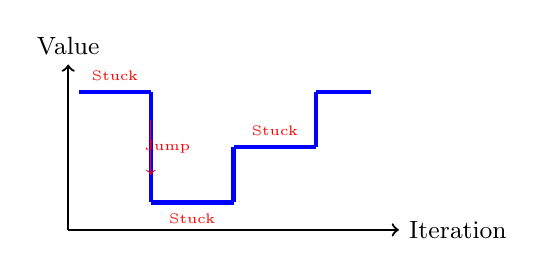
\begin{tikzpicture}[scale=0.7]
					\draw[thick, ->] (0,0) -- (6,0) node[right] {\small Iteration};
					\draw[thick, ->] (0,0) -- (0,3) node[above] {\small Value};

					% Metastable trajectory
					\draw[blue, ultra thick] (0.2, 2.5) -- (1.5, 2.5);
					\draw[blue, ultra thick] (1.5, 2.5) -- (1.5, 0.5);
					\draw[blue, ultra thick] (1.5, 0.5) -- (3, 0.5);
					\draw[blue, ultra thick] (3, 0.5) -- (3, 1.5);
					\draw[blue, ultra thick] (3, 1.5) -- (4.5, 1.5);
					\draw[blue, ultra thick] (4.5, 1.5) -- (4.5, 2.5);
					\draw[blue, ultra thick] (4.5, 2.5) -- (5.5, 2.5);

					% Annotations
					\node[red] at (0.85, 2.8) {\tiny Stuck};
					\node[red] at (2.25, 0.2) {\tiny Stuck};
					\node[red] at (3.75, 1.8) {\tiny Stuck};

					\draw[red, ->] (1.5, 2) -- (1.5, 1);
					\node[red] at (1.8, 1.5) {\tiny Jump};
				\end{tikzpicture}
			\end{center}

			Despite poor mixing:\\
			\begin{itemize}
				\item Similar means across chains
				\item Similar variances
				\item $\hat{R} \approx 1$
			\end{itemize}
		\end{column}
	\end{columns}
\end{frame}

\section{Best Practices}

\begin{frame}{Comprehensive Convergence Assessment}
	\begin{block}{Use Multiple Diagnostics}
		\begin{enumerate}
			\item \textbf{Gelman-Rubin statistic}: $\hat{R} < 1.01$
			\item \textbf{Effective Sample Size}: ESS $>$ 400 (minimum)
			\item \textbf{Trace plots}: Visual inspection
			\item \textbf{Autocorrelation}: Check mixing quality
			\item \textbf{Geweke test}: Compare chain beginning and end
		\end{enumerate}
	\end{block}

	\vspace{0.5cm}
	\textbf{Best Practices:}
	\begin{itemize}
		\item Use at least 4 chains (preferably more)
		\item Initialize chains from overdispersed starting points
		\item Run chains longer than you think necessary
		\item Use rank-normalized $\hat{R}$ (more robust)
		\item Check both bulk and tail $\hat{R}$
	\end{itemize}
\end{frame}

\begin{frame}{Modern Extensions}
	\begin{block}{Rank-Normalized $\hat{R}$ (Vehtari et al., 2021)}
		\begin{itemize}
			\item Transform samples to ranks (more robust to outliers)
			\item Split chains in half (detect within-chain problems)
			\item Separate bulk and tail diagnostics
		\end{itemize}
	\end{block}

	\vspace{0.5cm}
	\begin{columns}
		\begin{column}{0.5\textwidth}
			\textbf{Bulk-$\hat{R}$:}
			\begin{itemize}
				\item Convergence of center
				\item Mean, median
				\item Usually converges faster
			\end{itemize}
		\end{column}
		\begin{column}{0.5\textwidth}
			\textbf{Tail-$\hat{R}$:}
			\begin{itemize}
				\item Convergence of extremes
				\item 5\%, 95\% quantiles
				\item Needs more samples
			\end{itemize}
		\end{column}
	\end{columns}

	\vspace{0.5cm}
	\begin{center}
		\color{copenhagenred} Modern tools (Stan, ArviZ) implement these improvements
	\end{center}
\end{frame}

\begin{frame}{Summary Checklist}
	\begin{block}{MCMC Convergence Checklist}
		\begin{enumerate}
			\item Run at least 4 chains with dispersed starts
			\item Check $\hat{R} < 1.01$ for all parameters
			\item Verify ESS $>$ 400 (bulk and tail)
			\item Examine trace plots visually
			\item Check autocorrelation is low
			\item Run sensitivity analysis with different seeds
			\item Compare results from different samplers if possible
		\end{enumerate}
	\end{block}

	\vspace{0.5cm}
	\begin{center}
		\Large
		\textbf{Remember:}\\
		\vspace{0.3cm}
		\color{copenhagenred} No single diagnostic is perfect.\\
		Always use multiple checks!
	\end{center}
\end{frame}

\section{Conclusion}

\begin{frame}{Key Takeaways}
	\begin{enumerate}
		\item \textbf{Gelman-Rubin compares within vs between chain variance}
		      \begin{itemize}
			      \item Elegant idea: converged chains should agree
		      \end{itemize}

		\item \textbf{Modern threshold is $\hat{R} < 1.01$}
		      \begin{itemize}
			      \item Old threshold (1.1) gives only ~5 effective samples
			      \item New threshold ensures ~50 effective samples
		      \end{itemize}

		\item \textbf{$\hat{R}$ has important limitations}
		      \begin{itemize}
			      \item Can miss modes
			      \item Fooled by metastable states
			      \item Necessary but not sufficient
		      \end{itemize}

		\item \textbf{Always use multiple diagnostics}
		      \begin{itemize}
			      \item ESS, trace plots, autocorrelation
			      \item Visual inspection remains crucial
		      \end{itemize}
	\end{enumerate}

	\vspace{0.5cm}
	\begin{center}
		\Large \color{copenhagenred}
		Good MCMC diagnostics = Reliable scientific inference
	\end{center}
\end{frame}

\begin{frame}{References}
	\small
	\begin{itemize}
		\item Gelman, A. and Rubin, D.B. (1992). Inference from iterative simulation using multiple sequences. \textit{Statistical Science}, 7(4), 457-472.

		\item Gelman, A., et al. (2004). \textit{Bayesian Data Analysis} (2nd ed.). Chapman \& Hall/CRC.

		\item Vehtari, A., Gelman, A., Simpson, D., Carpenter, B., and Bürkner, P.C. (2021). Rank-normalization, folding, and localization: An improved $\hat{R}$ for assessing convergence of MCMC. \textit{Bayesian Analysis}, 16(2), 667-718.

		\item Vats, D. and Knudson, C. (2021). Revisiting the Gelman-Rubin diagnostic. \textit{Statistical Science}, 36(4), 518-529.

		\item Brooks, S.P. and Gelman, A. (1998). General methods for monitoring convergence of iterative simulations. \textit{Journal of Computational and Graphical Statistics}, 7(4), 434-455.
	\end{itemize}
\end{frame}

